%% 
%% Copyright 2007-2024 Elsevier Ltd
%% 
%% This file is part of the 'Elsarticle Bundle'.
%% ---------------------------------------------
%% 
%% It may be distributed under the conditions of the LaTeX Project Public
%% License, either version 1.3 of this license or (at your option) any
%% later version.  The latest version of this license is in
%%    http://www.latex-project.org/lppl.txt
%% and version 1.3 or later is part of all distributions of LaTeX
%% version 1999/12/01 or later.
%% 
%% The list of all files belonging to the 'Elsarticle Bundle' is
%% given in the file `manifest.txt'.
%% 
%% Template article for Elsevier's document class `elsarticle'
%% with harvard style bibliographic references

% \documentclass[preprint,12pt,authoryear]{elsarticle}

%% Use the option review to obtain double line spacing
% \documentclass[authoryear,preprint,review,12pt]{elsarticle}

%% Use the options 1p,twocolumn; 3p; 3p,twocolumn; 5p; or 5p,twocolumn
%% for a journal layout:
\documentclass[final,1p,times,authoryear]{elsarticle}
% \documentclass[final,1p,times,twocolumn,authoryear]{elsarticle}
%% \documentclass[final,3p,times,authoryear]{elsarticle}
%% \documentclass[final,3p,times,twocolumn,authoryear]{elsarticle}
%% \documentclass[final,5p,times,authoryear]{elsarticle}
%% \documentclass[final,5p,times,twocolumn,authoryear]{elsarticle}

%% For including figures, graphicx.sty has been loaded in
%% elsarticle.cls. If you prefer to use the old commands
%% please give \usepackage{epsfig}

%% The amssymb package provides various useful mathematical symbols
\usepackage{amssymb}
%% The amsmath package provides various useful equation environments.
\usepackage{amsmath}
%% The amsthm package provides extended theorem environments
%% \usepackage{amsthm}
% for tables
\usepackage{makecell}

\usepackage{hyperref}
\usepackage{longtable}
%% The lineno packages adds line numbers. Start line numbering with
%% \begin{linenumbers}, end it with \end{linenumbers}. Or switch it on
%% for the whole article with \linenumbers.
%% \usepackage{lineno}

\journal{eclinicalmedicine}

\begin{document}

\begin{frontmatter}

%% Title, authors and addresses

%% use the tnoteref command within \title for footnotes;
%% use the tnotetext command for theassociated footnote;
%% use the fnref command within \author or \affiliation for footnotes;
%% use the fntext command for theassociated footnote;
%% use the corref command within \author for corresponding author footnotes;
%% use the cortext command for theassociated footnote;
%% use the ead command for the email address,
%% and the form \ead[url] for the home page:
%% \title{Title\tnoteref{label1}}
%% \tnotetext[label1]{}
%% \author{Name\corref{cor1}\fnref{label2}}
%% \ead{email address}
%% \ead[url]{home page}
%% \fntext[label2]{}
%% \cortext[cor1]{}
%% \affiliation{organization={},
%%            addressline={}, 
%%            city={},
%%            postcode={}, 
%%            state={},
%%            country={}}
%% \fntext[label3]{}

\title{Machine learning model for predicting the visit duration of urticaria based on clinical laboratory data}

%% use optional labels to link authors explicitly to addresses:
%% \author[label1,label2]{}
%% \affiliation[label1]{organization={},
%%             addressline={},
%%             city={},
%%             postcode={},
%%             state={},
%%             country={}}
%%
%% \affiliation[label2]{organization={},
%%             addressline={},
%%             city={},
%%             postcode={},
%%             state={},
%%             country={}}

%% 作者和机构的对应关系通过label来实现
\author[XinHua]{Yijun Yang\fnref{fn1}}  % 第一位作者,属于两个机构
\author[XinHua]{Guofang Li\fnref{fn1}} 
\author[XinHua]{Zhen Zhang}
\author[XinHua]{Zhirong Yao}                            
\author[Jiuyuan]{Linting Huang\corref{cor2}}     
\author[XinHua]{Hui Zhang\corref{cor1}}                       
                                        
\cortext[cor1]{Corresponding author. Email: authora@example.com}  % 联系作者信息
\cortext[cor2]{Corresponding author. Email: huanglinting@163.com}  % 联系作者信息
\fntext[fn1]{Yijun Yang and Guofang Li contributed equally to this work.}  % 脚注信息


%% 机构1
\affiliation[XinHua]{organization={Shanghai XinHua Hospital affiliated to Shanghai Jiao Tong University School of Medicine},
            addressline={Address line of institution one},
            city={Shanghai},
            postcode={200092},
            state={Shanghai},
            country={China}}

%% 机构2
\affiliation[Jiuyuan]{organization={The ninth hospital of Shanghai Jiao Tong University School of Medicine},
            addressline={Address line of institution two},
            city={Shanghai},
            postcode={200011},
            state={Shanghai},
            country={China}}


%% Abstract
\begin{abstract}
%% Text of abstract
Background: Urticaria is a common condition presenting with wheals, angioedema, or both, driven by mast cell degranulation. The duration of urticaria, particularly chronic spontaneous urticaria (CSU), is crucial for effective patient management and treatment planning. This study aimed to build a machine learning model for predicting the visit duration of urticaria based on clinical laboratory data and to identify the factors that contribute to prolonged episodes of chronic urticaria.

Method: 

Results:

Conclusion: 
\end{abstract}

%%Graphical abstract
% \begin{graphicalabstract}
% %\includegraphics{grabs}
% \end{graphicalabstract}

%%Research highlights
\begin{highlights}
\item A machine learning model was built to predict the visit duration of urticaria based on clinical laboratory data.
\item Inversed trend of shapley values of laboratory data in different phase of disease was observed.
\end{highlights}

%% Keywords
\begin{keyword}
%% keywords here, in the form: keyword \sep keyword

%% PACS codes here, in the form: \PACS code \sep code

%% MSC codes here, in the form: \MSC code \sep code
%% or \MSC[2008] code \sep code (2000 is the default)

\end{keyword}

\end{frontmatter}

%% Add \usepackage{lineno} before \begin{document} and uncomment 
%% following line to enable line numbers
%% \linenumbers

%% main text
\sloppy %% Allow LaTeX to stretch lines and break words to prevent overfull hbox

\section{Introduction}\label{Introduction}

Urticaria is a common condition presenting with wheals, angioedema, or both, driven by mast cell degranulation\citep{Zuberbier2021The,RadonjicHoesli2018Urticaria,Ring2012Urticaria}. The lifetime prevalence for acute urticaria is approximately 20\% \citep{Zuberbier2021The}. 

Urticaria is classified based on duration and triggers. Acute urticaria lasts less than 6 weeks, often triggered by specific causes like drugs, food, or infections. While chronic urticaria lasts more than 6 weeks and can be further classified into chronic spontaneous urticaria (CSU) and chronic inducible urticaria (CIndU)\citep{Zuberbier2021The,Ring2012Urticaria}. 

CSU is characterized by the spontaneous occurrence of wheals and/or angioedema without a specific trigger and often associated with autoimmune mechanisms\citep{Schettini2023Urticaria}, while CIndU is triggered by specific stimuli like cold, heat, or pressure\citep{Pozderac2020Chronic}. 

The prevalence of CSU is approximately 0.5\% in general population, and is less prevalent in children compared to adults\citep{Balp2015The, Poddighe2019LETTER, Labbene2023Prevalence}. Some patients with CSU experience trigger-induced wheals, angioedema, or both. Up to 36\% of patients with CSU have been reported to react concomitantly to physical trigger tests\citep{Dressler2018Chronic}. These triggers are not definite, as their presence does not always induce signs and symptoms and because wheals, angioedema, or both also occur without them, that is, spontaneously. Some patients can present with more than one subtype of urticaria\citep{Zuberbier2021The}. 

Chronic urticaria significantly impairs quality of life, affecting work and school performance. It is considered a severe allergic disease due to its disabling nature and high disease burden\citep{Zuberbier2021The}. Duration of CSU greater than 3 years are associated with better responses to second-generation antihistamines and other treatments\citep{Chiang2022Predictors}. Predicting the duration of urticaria, particularly chronic spontaneous urticaria (CSU), is crucial for effective patient management and treatment planning. 

Several clinical features have been associated with the severity and duration of chronic spontaneous urticaria (CSU). Higher age at onset, female gender, longer disease duration, and hypersensitivity to aspirin or nonsteroidal anti-inflammatory drugs (NSAIDs) are linked to more severe CSU and prolonged time to remission \citep{SanchezBorges2017Factors,Rabelo-Filardi2013Parameters}. Patients exhibiting concomitant CIndU and recurrent angioedema also tend to experience longer durations of CSU \citep{SanchezBorges2017Factors, Curto-Barredo2018Clinical}. Moreover, patients with multiple allergic conditions are more likely to have prolonged episodes of urticaria \citep{Lin2011Predictive}.

Potential biomarkers for CSU severity and duration have been identified. Positive autologous serum skin test (ASST) results, basophil counts, levels of inflammatory markers, activation markers of the extrinsic coagulation pathway, immunoglobulin E (IgE), and vitamin D levels are all associated with the disease's severity and duration \citep{SanchezBorges2017Factors,Rabelo-Filardi2013Parameters}. Specifically, plasma levels of prothrombin fragment, D-dimer, and C-reactive protein (CRP) may serve as markers of CSU severity \citep{Rabelo-Filardi2013Parameters}. Serum diamine oxidase (DAO) levels have been linked to the response to antihistamines and dietary interventions, indicating a potential role in predicting disease duration \citep{Chiang2022Predictors}.

Metabolic factors also play a role, with high waist circumference (WC), rather than high body mass index (BMI), emerging as a predictive risk factor for longer disease duration in CSU patients \citep{Kim2021High}.

The aim of this study was to build a machine learning model for predicting the visit duration of urticaria based on clinical laboratory data and to identify the factors can contribute to prolonged episodes of chronic urticaria by analyzing the importance of variables in the model, hoping to provide a reference for the clinical management of urticaria.

\section{Methods}\label{Methods}
%% Use \subsection commands to start a subsection.
\subsection{Patients}\label{Patients}

patients with urticaria were recruited from the urticaria specialty clinic of the dermatology department of Shanghai XinHua Hospital affiliated to Shanghai Jiao Tong University School of Medicine from January 2018 to December 2024. The inclusion criteria were as follows: (1) patients diagnosed with urticaria according to the EAACI/GA2LEN/EDF/WAO guidelines\citep{Zuberbier2021The}; (2) patients with complete clinical and laboratory data; (3) patients with stable follow-up history, indicated by at least 3 times of follow-up visits. the exclusion criteria were as follows: (1) patients with other skin diseases; (2) patients with severe systemic diseases; (3) patients with incomplete clinical data. The study was approved by the ethics committee of Shanghai XinHua Hospital affiliated to Shanghai Jiao Tong University School of Medicine, and all patients provided written informed consent.

\subsection{Data collection and management}\label{Data}

the data of patients with urticaria were collected from the electronic medical record system of the hospital, including demographic data, clinical data, laboratory data. the data were stored in a mysql database for subsequent analysis as follows: (1) Patients: containing basic information of each unique patient; (2) OutpatientNumbers: storing relationship between outpatient numbers with unique patient; (3) PatientVisits: containing visit events records; (4) PatientExaminations: containing the examination events records; (5) ExaminationItems: a dictionary table describing the examination items. the database schema is shown in database. Database 
markup language (DBML) describing the database schema is shown in supplementary materials.


\subsection{Feature extraction and feature engineering}\label{FeatureEngineering}
Visit duration, calculated by the difference between the first visit date and the last visit date, was the target variable. The following features were extracted from the database: (1) demographic data: gender, first visit age; (2) clinical data: concomitant inducible urticaria; (3) laboratory data: results from common blood tests, CRP, immunoglobulin, 25-hydroxyvitamin D, Thyroid function, autoantibodies, coagulation function, common urine tests, and allergen specific IgE tests. 
For laboratory data, 2 types of data were extracted: time-independent data and time-dependent data. Time-independent data are average values of laboratory data during the whole follow-up period, while time-dependent data are average values of laboratory data durting preclincial phase (before the onset of urticaria), acute phase (within 6 weeks after the onset of urticaria), and chronic phase (after 6 weeks of the onset of urticaria). 2 datasets were generated: one with time-independent data and one with time-dependent data, and were compared for prediction performance in the model development process. The sql queries for data are shown in feature\_extraction.sql in supplementary materials. 

\subsection{Model development and comparison}\label{Training}
Dataset was split into training set and test set with a ratio of 7:3. 5 models were adopted for comparison: Xgboost, random forest, adaboost, gradient boosting machine (GBM), and support vector machine (SVM). Hyperparameter optimization was performed using TPE algorithm by nni package in python, which is a bayesian optimization algorithm that uses tree-structured parzen estimator to model the objective function and suggest the next set of hyperparameters to evaluate based on the previous results. Internal 5 fold cross-validation was employed to discern the most suitable hyperparameters for each distinct model, individually applied to each model for enhanced performance. The performance of the model and data was evaluated by receiver operating characteristic (ROC) curve, area under the curve (AUC), accuracy, precision, recall and F1 score on different cuttoffs of disease duration. The sensitivity, specificity, PPV, NPV, accuracy, and F1 score were calculated at the optimal cutoff value that maximized the Youden index. The model and data with the best performance were selected for further analysis.


\subsection{feature selection}\label{FeatureSelection}

Too many features can lead to overfitting and reduce the interpretability of the model. Therefore, feature selection was performed on final model for further optimization. Although, feature importances can be evalutated directly from the boosted trees, these importances have been shown to be local and inconsistent. A SHAP score inspired by Shapley values can combines different explanation models and provide a global feature importance score that is consistent across different test sets. However, other than to arbitrarily select an importance threshold beyond which features are considered unimportant, SHAP analysis does not offer an algorithmic way to filter a large feature set to a limited set of important features. Boruta algorithm is a wrapper method that determine the importance of features by comparing the importance of original features with their shuffled copies, If importance of an original feature is significantly greater than its shuffled copy, that features is deemed important. 

In this study, Boruta algorithm was run on the final model, with max iteration set to 50 and repeated 15 times.
The confirmed features list and importance rank were recorded for each run. The overlap of confirmed features across runs was calculated to determine the final feature list. For time dependent data, once a laboratory item was confirmed as important in any phase of disease, the feature of the same lab item in other phase of disease was also considered as important. That is to say, when top 10 items were selected, the features representing different phases of that item were all included in the final model, which is at most 30 features for time dependent data. The model performance on different number of top items, ranked by the average importance score, were compared to determine the optimal number of features for the final model.


\subsection{Model explanation}\label{ModelExplanationMethods}

The shapley value of each laboratory item in different phase of disease were compared to reveal various predicting ability of laboratory data in different phase of disease. To further verify the tendency oberserved in shapley values, kernal density estimation was used to visualize the distribution of average values of laboratory data in different phase of disease for patients with different disease duration. Shapley values together with kernal density estimation were used to explain the model and provide insights for clinical practice. Some of the features were further analyzed with different age populations to explore the potential age effect on the predicting ability of laboratory data.


\section{Results}\label{Results}

\subsection{Patient characteristics}\label{PatientCharacteristics}

Table \ref{tab:good_outcome_poor_outcome_origi} and Table \ref{tab:good_outcome_poor_outcome_time} delineates the disparities between groups regarding the disease duration of patients in dataset. 

Table \ref{tab:train_test_origi} and table \ref{tab:train_test_time} provides a comparison of the baseline characteristic between the training set and external testing set data. No substantial differences were observed between the training set and the external test set across the majority of features in either time independent or time dependent data.
\begin{table}[htbp]\centering\begin{tabular}{lccc}\hline
Characteristic & Good Outcome & Poor Outcome & P-value \\
\hline
Number of patients & 2027 & 1927 & \\

\makecell[l]{Outcome} & $25.37 \pm 25.09$ & $604.32 \pm 437.04$ & 0.000 $\uparrow$ \\

\makecell[l]{Gender} & 0: 64.7\%, 1: 35.3\% & 0: 61.1\%, 1: 38.9\% & 0.023  \\

\makecell[l]{First Visit Age} & $30.12 \pm 21.79$ & $28.11 \pm 23.61$ & 0.005 $\downarrow$ \\

\makecell[l]{CI nd U} & 0: 99.3\%, 1: 0.7\% & 0: 97.2\%, 1: 2.8\% & 0.000  \\

\makecell[l]{Lymphocytes Percentage} & $28.98 \pm 14.05$ & $34.02 \pm 13.88$ & 0.000 $\uparrow$ \\

\makecell[l]{Neutrophils Percentage} & $63.13 \pm 15.68$ & $56.63 \pm 14.97$ & 0.000 $\downarrow$ \\

\makecell[l]{Monocytes Percentage} & $6.18 \pm 1.64$ & $6.49 \pm 1.67$ & 0.000 $\uparrow$ \\

\makecell[l]{Mean Corpuscular \\ Hemoglobin \\ Concentration} & $335.62 \pm 10.51$ & $336.93 \pm 10.30$ & 0.000 $\uparrow$ \\

\makecell[l]{Platelet Count} & $263.47 \pm 74.09$ & $256.73 \pm 68.96$ & 0.003 $\downarrow$ \\

\makecell[l]{White Blood Cell Count} & $10.31 \pm 3.00$ & $9.35 \pm 2.39$ & 0.000 $\downarrow$ \\

\makecell[l]{Mean Corpuscular \\ Hemoglobin} & $29.07 \pm 2.33$ & $28.98 \pm 2.30$ & 0.202  \\

\makecell[l]{Mean Corpuscular Volume} & $86.66 \pm 6.65$ & $85.99 \pm 6.67$ & 0.002 $\downarrow$ \\

\makecell[l]{Hemoglobin} & $130.03 \pm 9.16$ & $130.20 \pm 8.46$ & 0.546  \\

\makecell[l]{Eosinophils Percentage} & $1.55 \pm 2.02$ & $2.31 \pm 2.37$ & 0.000 $\uparrow$ \\

\makecell[l]{Basophils Percentage} & $0.25 \pm 0.22$ & $0.32 \pm 0.24$ & 0.000 $\uparrow$ \\

\makecell[l]{Absolute Eosinophil \\ Count} & $0.13 \pm 0.20$ & $0.18 \pm 0.21$ & 0.000 $\uparrow$ \\

\makecell[l]{Absolute Lymphocyte \\ Count} & $2.61 \pm 1.12$ & $2.83 \pm 1.29$ & 0.000 $\uparrow$ \\

\makecell[l]{Mean Platelet Volume} & $9.14 \pm 1.39$ & $9.02 \pm 1.39$ & 0.007 $\downarrow$ \\

\makecell[l]{Platelet Distribution \\ Width} & $12.72 \pm 1.96$ & $12.57 \pm 1.94$ & 0.020  \\

\makecell[l]{Eosinophil Count \\ Absolute} & $128.60 \pm 141.68$ & $162.83 \pm 190.02$ & 0.000 $\uparrow$ \\

\makecell[l]{CR eactive Protein} & $13.03 \pm 19.62$ & $7.71 \pm 10.23$ & 0.000 $\downarrow$ \\

\makecell[l]{Immunoglobulin E} & $131.65 \pm 242.00$ & $152.28 \pm 346.75$ & 0.029  \\

\makecell[l]{SMRNP} & $1.18 \pm 2.16$ & $1.22 \pm 1.84$ & 0.576  \\

\makecell[l]{Anti SSA} & $1.42 \pm 5.44$ & $1.58 \pm 5.68$ & 0.363  \\

\makecell[l]{Anti Jo 1} & $1.08 \pm 1.77$ & $1.12 \pm 2.06$ & 0.534  \\

\makecell[l]{Nucleosome} & $0.57 \pm 0.34$ & $0.65 \pm 0.43$ & 0.000 $\uparrow$ \\

\makecell[l]{Ribosomal PP rotein} & $1.07 \pm 0.71$ & $1.17 \pm 2.13$ & 0.050  \\

\makecell[l]{Ro 52} & $2.10 \pm 5.90$ & $2.23 \pm 6.81$ & 0.515  \\
\hline\end{tabular}\caption{Comparison of the characteristics between patients with good and poor outcomes in the time independent dataset \\ continuous variables are presented as mean ± standard deviation, categorical variables are presented as number (percentage) \\ good outcome is defined as visit duration < 100 days, poor outcome is defined as visit duration $\geq$ 100 days} \label{tab:good_outcome_poor_outcome_origi}
\end{table}
\begin{table}[htbp]\centering\begin{tabular}{lccc}\hline
Characteristic & Good Outcome & Poor Outcome & P-value \\
\hline
Number of patients & 1202 & 746 & \\

\makecell[l]{Outcome} & $14.68 \pm 22.61$ & $631.42 \pm 448.34$ & 0.000 $\uparrow$ \\

\makecell[l]{Gender} & 0: 84.6\%, 1: 15.4\% & 0: 77.3\%, 1: 22.7\% & 0.000  \\

\makecell[l]{First Visit Age} & $22.60 \pm 21.58$ & $22.26 \pm 23.12$ & 0.746  \\

\makecell[l]{CI nd U} & 0: 99.4\%, 1: 0.6\% & 0: 98.5\%, 1: 1.5\% & 0.079  \\

\makecell[l]{Lymphocytes Percentage \\ preclinical} & $37.86 \pm 14.45$ & $40.34 \pm 15.16$ & 0.000 $\uparrow$ \\

\makecell[l]{Lymphocytes Percentage \\ chronic} & $35.37 \pm 9.29$ & $36.50 \pm 11.95$ & 0.019 $\uparrow$ \\

\makecell[l]{Lymphocytes Percentage \\ acute} & $32.37 \pm 14.25$ & $34.65 \pm 13.91$ & 0.001 $\uparrow$ \\

\makecell[l]{Neutrophils Percentage \\ chronic} & $54.34 \pm 10.18$ & $53.71 \pm 12.76$ & 0.229  \\

\makecell[l]{Neutrophils Percentage \\ acute} & $59.48 \pm 15.77$ & $56.92 \pm 14.85$ & 0.000 $\downarrow$ \\

\makecell[l]{Neutrophils Percentage \\ preclinical} & $51.40 \pm 15.89$ & $48.94 \pm 16.49$ & 0.001 $\downarrow$ \\

\makecell[l]{Monocytes Percentage \\ acute} & $6.23 \pm 1.08$ & $6.23 \pm 1.04$ & 0.937  \\

\makecell[l]{Monocytes Percentage \\ chronic} & $6.53 \pm 0.77$ & $6.53 \pm 1.22$ & 0.980  \\

\makecell[l]{Monocytes Percentage \\ preclinical} & $6.66 \pm 1.03$ & $6.70 \pm 0.82$ & 0.359  \\

\makecell[l]{Mean Corpuscular \\ Hemoglobin \\ Concentration acute} & $336.49 \pm 12.49$ & $338.59 \pm 12.85$ & 0.000 $\uparrow$ \\

\makecell[l]{Mean Corpuscular \\ Hemoglobin \\ Concentration chronic} & $333.82 \pm 4.53$ & $334.04 \pm 8.74$ & 0.457  \\

\makecell[l]{Mean Corpuscular \\ Hemoglobin \\ Concentration \\ preclinical} & $343.26 \pm 6.90$ & $343.88 \pm 7.38$ & 0.058  \\

\makecell[l]{Platelet Count acute} & $260.29 \pm 69.51$ & $258.81 \pm 62.12$ & 0.634  \\

\makecell[l]{Platelet Count chronic} & $253.50 \pm 31.29$ & $257.54 \pm 57.28$ & 0.044 $\uparrow$ \\

\makecell[l]{Platelet Count \\ preclinical} & $252.05 \pm 52.40$ & $255.30 \pm 50.00$ & 0.176  \\

\makecell[l]{White Blood Cell Count \\ acute} & $10.06 \pm 3.20$ & $9.56 \pm 2.56$ & 0.000 $\downarrow$ \\

\makecell[l]{White Blood Cell Count \\ preclinical} & $8.65 \pm 2.05$ & $8.52 \pm 1.81$ & 0.179  \\

\makecell[l]{White Blood Cell Count \\ chronic} & $8.44 \pm 1.00$ & $8.67 \pm 2.31$ & 0.003 $\uparrow$ \\

\makecell[l]{Mean Corpuscular \\ Hemoglobin preclinical} & $28.47 \pm 1.63$ & $28.30 \pm 1.73$ & 0.027 $\downarrow$ \\

\makecell[l]{Mean Corpuscular \\ Hemoglobin acute} & $28.60 \pm 2.03$ & $28.64 \pm 2.04$ & 0.686  \\

\makecell[l]{Mean Corpuscular \\ Hemoglobin chronic} & $28.93 \pm 1.41$ & $28.79 \pm 1.75$ & 0.064  \\

\makecell[l]{Mean Corpuscular Volume \\ acute} & $85.02 \pm 6.22$ & $84.57 \pm 5.81$ & 0.113  \\

\makecell[l]{Mean Corpuscular Volume \\ preclinical} & $83.11 \pm 5.43$ & $82.44 \pm 5.83$ & 0.010 $\downarrow$ \\

\makecell[l]{Mean Corpuscular Volume \\ chronic} & $86.62 \pm 4.32$ & $86.02 \pm 5.27$ & 0.006 $\downarrow$ \\

\makecell[l]{Hemoglobin acute} & $129.24 \pm 9.96$ & $129.41 \pm 7.91$ & 0.690  \\

\makecell[l]{Hemoglobin preclinical} & $128.17 \pm 7.15$ & $127.20 \pm 8.29$ & 0.006 $\downarrow$ \\

\makecell[l]{Hemoglobin chronic} & $130.22 \pm 4.78$ & $129.84 \pm 7.44$ & 0.171  \\

\makecell[l]{Eosinophils Percentage \\ preclinical} & $2.74 \pm 2.57$ & $2.74 \pm 2.41$ & 0.982  \\

\makecell[l]{Eosinophils Percentage \\ chronic} & $2.28 \pm 1.31$ & $2.29 \pm 1.87$ & 0.874  \\

\makecell[l]{Eosinophils Percentage \\ acute} & $1.71 \pm 2.28$ & $1.60 \pm 1.71$ & 0.217  \\

\makecell[l]{Basophils Percentage \\ acute} & $0.22 \pm 0.19$ & $0.22 \pm 0.17$ & 0.781  \\

\makecell[l]{Basophils Percentage \\ preclinical} & $0.27 \pm 0.13$ & $0.27 \pm 0.14$ & 0.872  \\

\makecell[l]{Basophils Percentage \\ chronic} & $0.30 \pm 0.13$ & $0.30 \pm 0.21$ & 1.000  \\

\makecell[l]{Absolute Eosinophil \\ Count preclinical} & $0.22 \pm 0.33$ & $0.23 \pm 0.31$ & 0.729  \\

\makecell[l]{Absolute Eosinophil \\ Count acute} & $0.15 \pm 0.24$ & $0.14 \pm 0.16$ & 0.215  \\

\makecell[l]{Absolute Eosinophil \\ Count chronic} & $0.18 \pm 0.11$ & $0.18 \pm 0.16$ & 0.513  \\

\makecell[l]{Absolute Lymphocyte \\ Count acute} & $2.96 \pm 1.30$ & $3.03 \pm 1.29$ & 0.268  \\

\makecell[l]{Absolute Lymphocyte \\ Count preclinical} & $3.13 \pm 1.27$ & $3.35 \pm 1.44$ & 0.001 $\uparrow$ \\

\makecell[l]{Absolute Lymphocyte \\ Count chronic} & $2.68 \pm 0.85$ & $2.85 \pm 1.10$ & 0.000 $\uparrow$ \\

\makecell[l]{Mean Platelet Volume \\ preclinical} & $9.55 \pm 0.84$ & $9.51 \pm 0.79$ & 0.328  \\

\makecell[l]{Mean Platelet Volume \\ chronic} & $9.10 \pm 0.87$ & $9.21 \pm 1.21$ & 0.023 $\uparrow$ \\

\makecell[l]{Mean Platelet Volume \\ acute} & $9.85 \pm 1.14$ & $9.60 \pm 1.10$ & 0.000 $\downarrow$ \\

\makecell[l]{Platelet Distribution \\ Width acute} & $12.02 \pm 2.01$ & $11.85 \pm 1.79$ & 0.055  \\

\makecell[l]{Platelet Distribution \\ Width preclinical} & $11.88 \pm 1.47$ & $11.75 \pm 1.60$ & 0.063  \\

\makecell[l]{Platelet Distribution \\ Width chronic} & $12.05 \pm 1.16$ & $12.05 \pm 1.74$ & 0.973  \\

\makecell[l]{Eosinophil Count \\ Absolute preclinical} & $227.46 \pm 179.57$ & $246.76 \pm 272.94$ & 0.060  \\

\makecell[l]{Eosinophil Count \\ Absolute chronic} & $176.85 \pm 87.01$ & $183.78 \pm 140.98$ & 0.180  \\

\makecell[l]{Eosinophil Count \\ Absolute acute} & $126.66 \pm 129.69$ & $124.36 \pm 126.04$ & 0.700  \\

\makecell[l]{CR eactive Protein \\ chronic} & $5.39 \pm 4.84$ & $6.47 \pm 8.81$ & 0.000 $\uparrow$ \\

\makecell[l]{CR eactive Protein \\ preclinical} & $9.01 \pm 7.67$ & $8.81 \pm 7.16$ & 0.565  \\

\makecell[l]{CR eactive Protein \\ acute} & $10.21 \pm 10.95$ & $8.95 \pm 8.22$ & 0.007 $\downarrow$ \\

\makecell[l]{Immunoglobulin E \\ chronic} & $218.43 \pm 162.64$ & $219.37 \pm 444.66$ & 0.947  \\

\makecell[l]{Immunoglobulin E acute} & $149.91 \pm 107.06$ & $166.20 \pm 113.25$ & 0.001 $\uparrow$ \\

\makecell[l]{Free Thyroxine acute} & $15.40 \pm 0.76$ & $15.31 \pm 0.79$ & 0.012 $\downarrow$ \\

\makecell[l]{Free Thyroxine chronic} & $16.15 \pm 0.83$ & $16.21 \pm 1.04$ & 0.147  \\

\makecell[l]{SMRNP chronic} & $1.24 \pm 1.70$ & $1.24 \pm 0.68$ & 0.987  \\

\makecell[l]{SMRNP acute} & $1.32 \pm 0.70$ & $1.38 \pm 0.59$ & 0.061  \\

\makecell[l]{Anti SSA acute} & $1.11 \pm 2.90$ & $1.26 \pm 4.29$ & 0.364  \\

\makecell[l]{Anti SSA chronic} & $1.29 \pm 2.79$ & $1.40 \pm 2.79$ & 0.400  \\

\makecell[l]{Anti Jo 1 acute} & $0.82 \pm 0.44$ & $0.84 \pm 0.43$ & 0.356  \\

\makecell[l]{Anti Jo 1 chronic} & $1.07 \pm 0.99$ & $1.06 \pm 0.45$ & 0.909  \\

\makecell[l]{Nucleosome acute} & $1.14 \pm 0.75$ & $1.12 \pm 0.72$ & 0.528  \\

\makecell[l]{Nucleosome chronic} & $0.53 \pm 0.43$ & $0.54 \pm 0.46$ & 0.388  \\

\makecell[l]{Ribosomal PP rotein \\ acute} & $1.08 \pm 0.27$ & $1.10 \pm 0.29$ & 0.217  \\

\makecell[l]{Ribosomal PP rotein \\ chronic} & $1.15 \pm 0.23$ & $1.30 \pm 3.20$ & 0.117  \\

\makecell[l]{Ro 52 chronic} & $1.79 \pm 1.92$ & $1.92 \pm 3.52$ & 0.304  \\

\makecell[l]{Ro 52 acute} & $1.79 \pm 2.05$ & $1.91 \pm 4.32$ & 0.425  \\
\hline\end{tabular}\caption{Comparison of the characteristics between patients with good and poor outcomes in the time dependent dataset \\ continuous variables are presented as mean ± standard deviation, categorical variables are presented as number (percentage) \\ good outcome is defined as visit duration < 100 days, poor outcome is defined as visit duration $\geq$ 100 days} \label{tab:good_outcome_poor_outcome_time}
\end{table}

\subsection{Comparison of multiple models on time-dependent and time-independent data}\label{ModelComparison}
% xgboost + time dependent datasset is the best model in 42 100 365 cutoffs

Time independent and Time dependent data were used to generate 5 machine learning models to predict the disease duration of urticaria. Among the 10 models, Xgboost model with time dependent data (AUC = )  has the best predictive effect for disease duration, followed by random forest with time dependent data (AUC = ) the ROC curves for the top three best-performing ML models are presented in Figure \ref{Figure1}. The discriminative performances and ROC curves of all 10 models are listed in Supplementary Table \ref{tab:kfold_results}, and Supplementary Figure \ref{fig:kfold_all}, respectively.

% insert image
\begin{figure}[t]%% placement specifier
    %% Use \includegraphics command to insert graphic files. Place graphics files in 
    %% working directory.
    \centering%% For centre alignment of image.
    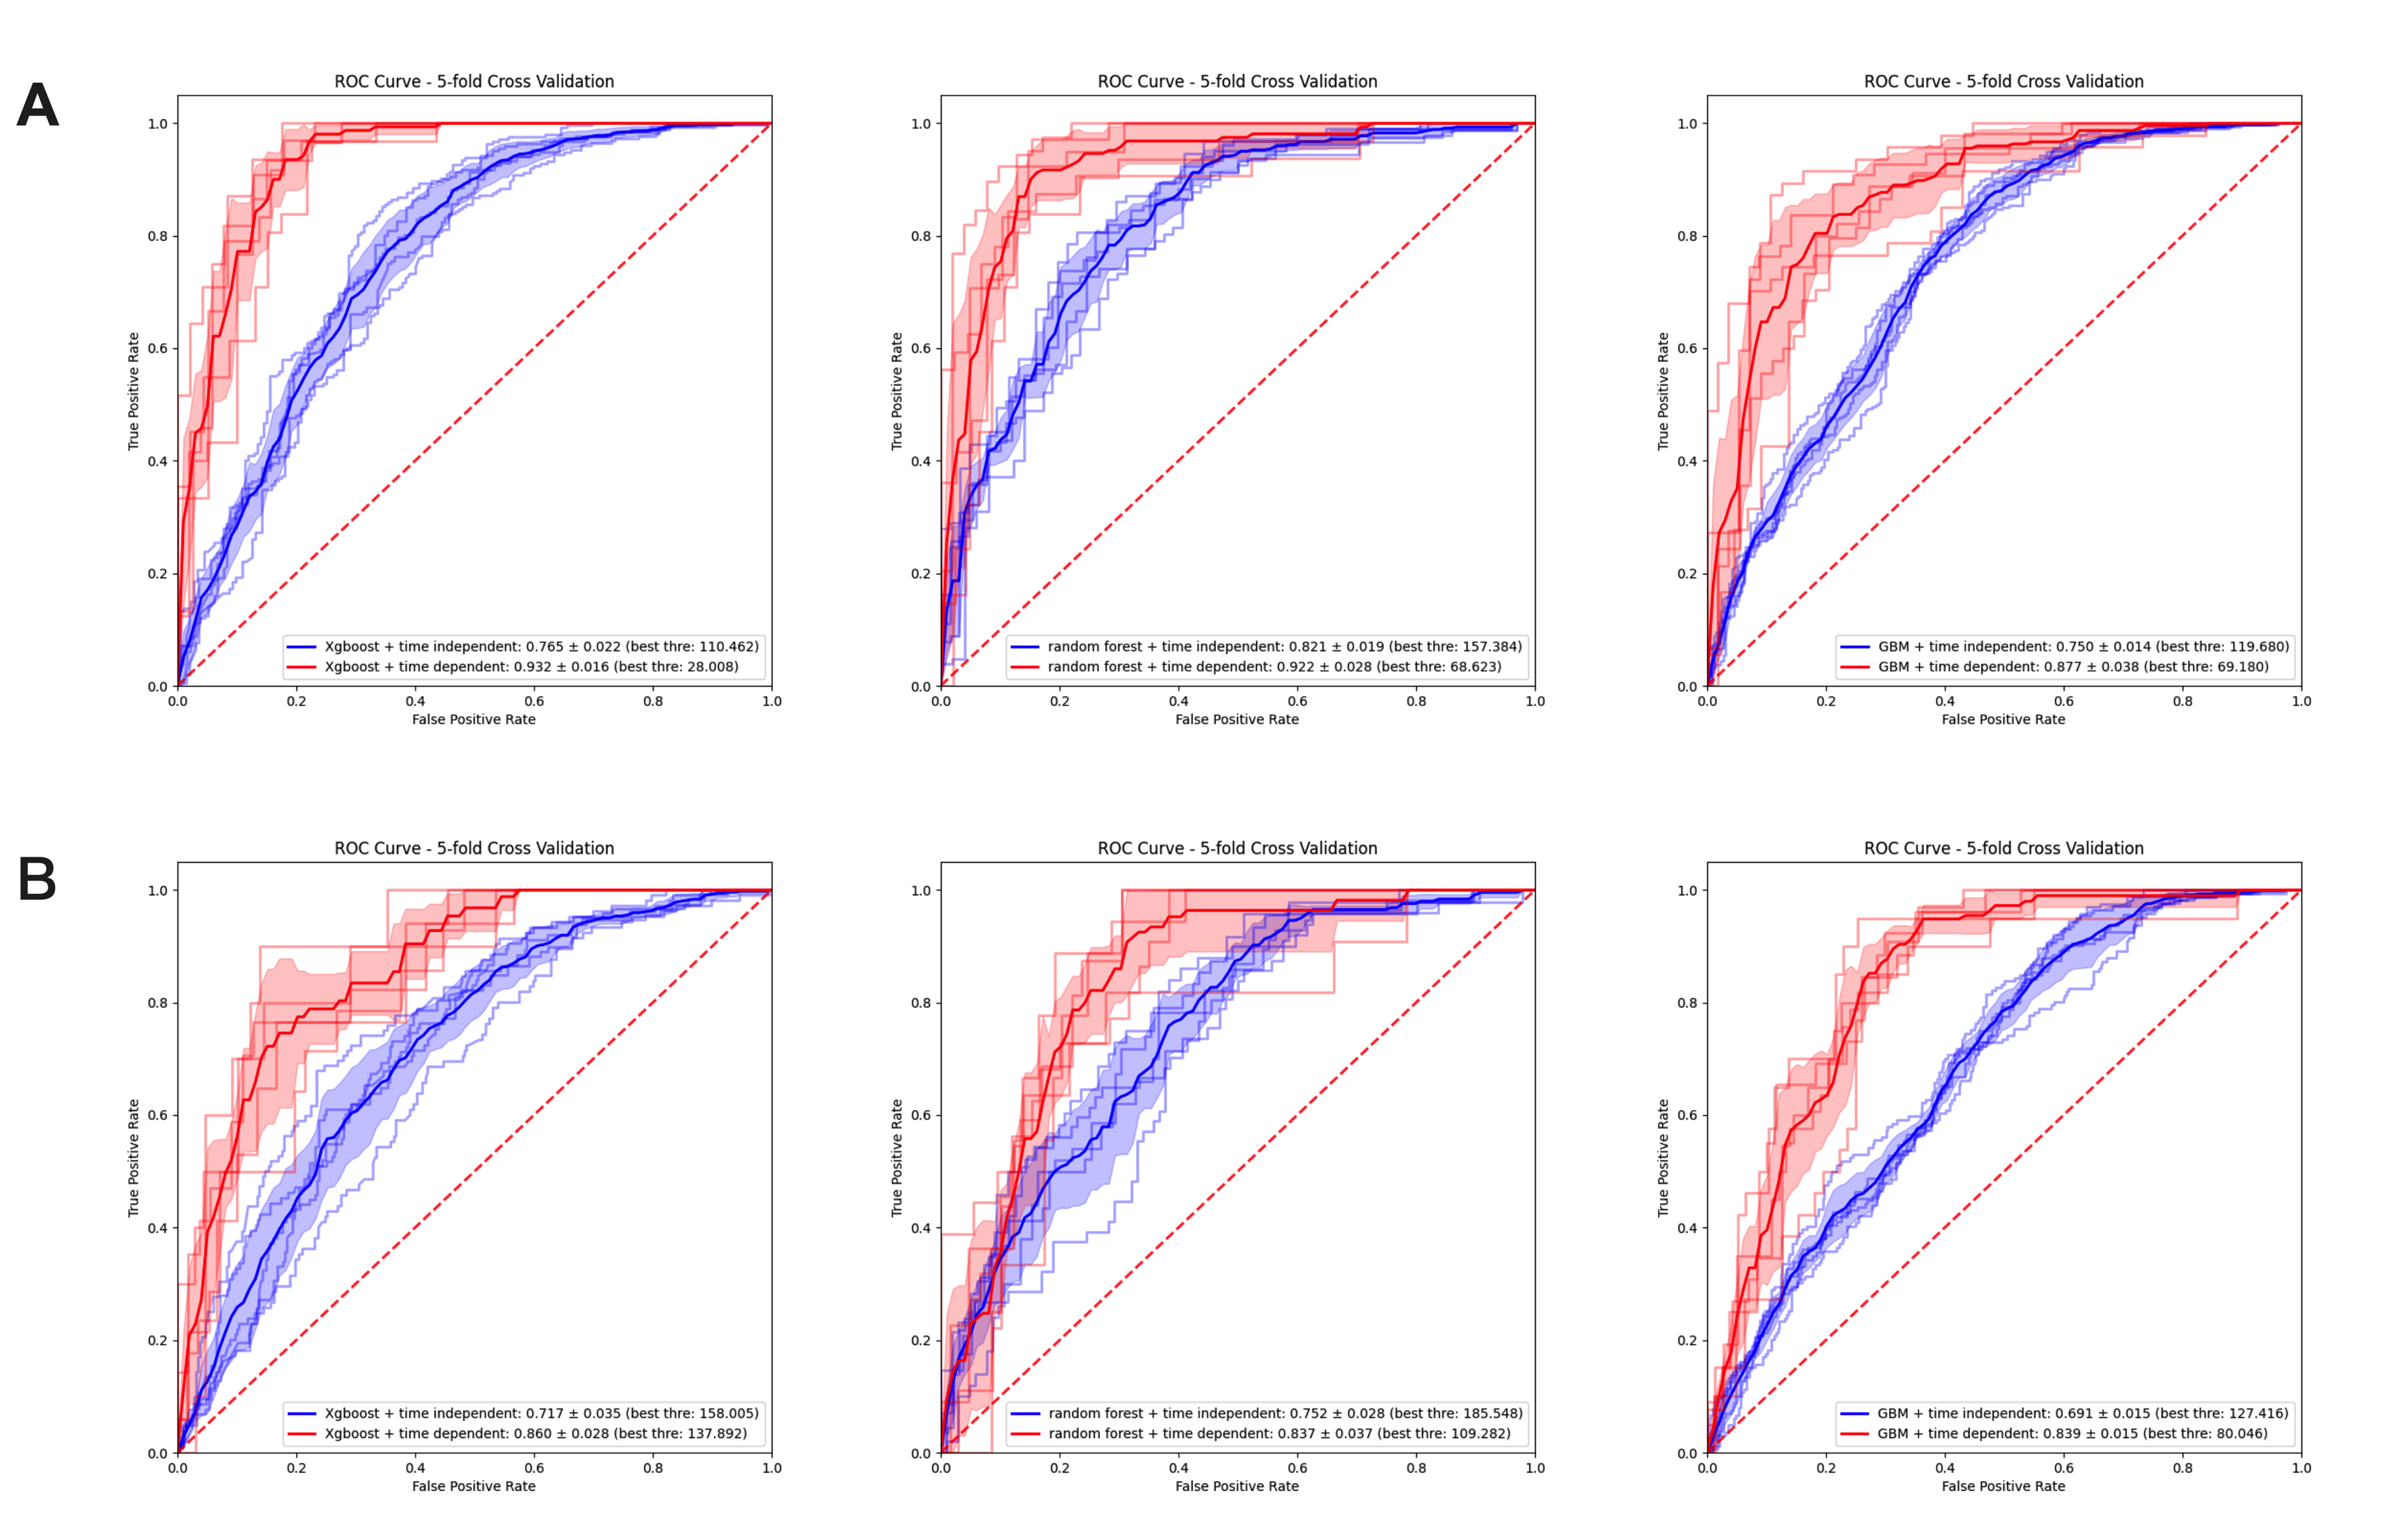
\includegraphics[width=\textwidth]{figures/kfoldfirst3.png}
    %% Use \caption command for figure caption and label.
    \caption{Figure Caption}\label{Figure1}
    %% https://en.wikibooks.org/wiki/LaTeX/Importing_Graphics#Importing_external_graphics
\end{figure}


\subsection{Feature selection and final model}\label{FinalModel}

Xgboost with time dependent data, as the best performing model, was selected for further optimization. Feature importance ranking by Boruta algorithm are shown in Figure \ref{Figure2} and Supplementary Table \ref{tab:boruta_ranking_df}. A total of 38 laboratory items were confirmed as important by Boruta algorithm, as shown in Supplementary Table \ref{tab:boruta_confirmed_vars}.

During the process of reducing features based on the feature important ranking, the changes in AUCs for the model shows that the model maintain robust performance unitil the number of items reduced to less than 10, as shown in Figure \ref{Figure3} A-C. Top 25 items were selected as the final model, validation on external test set showed a stable performance with AUC of 0.85, as shown in Figure 3 \ref{Figure3} D-F.


% insert image
\begin{figure}[t]%% placement specifier
    %% Use \includegraphics command to insert graphic files. Place graphics files in 
    %% working directory.
    \centering%% For centre alignment of image.
    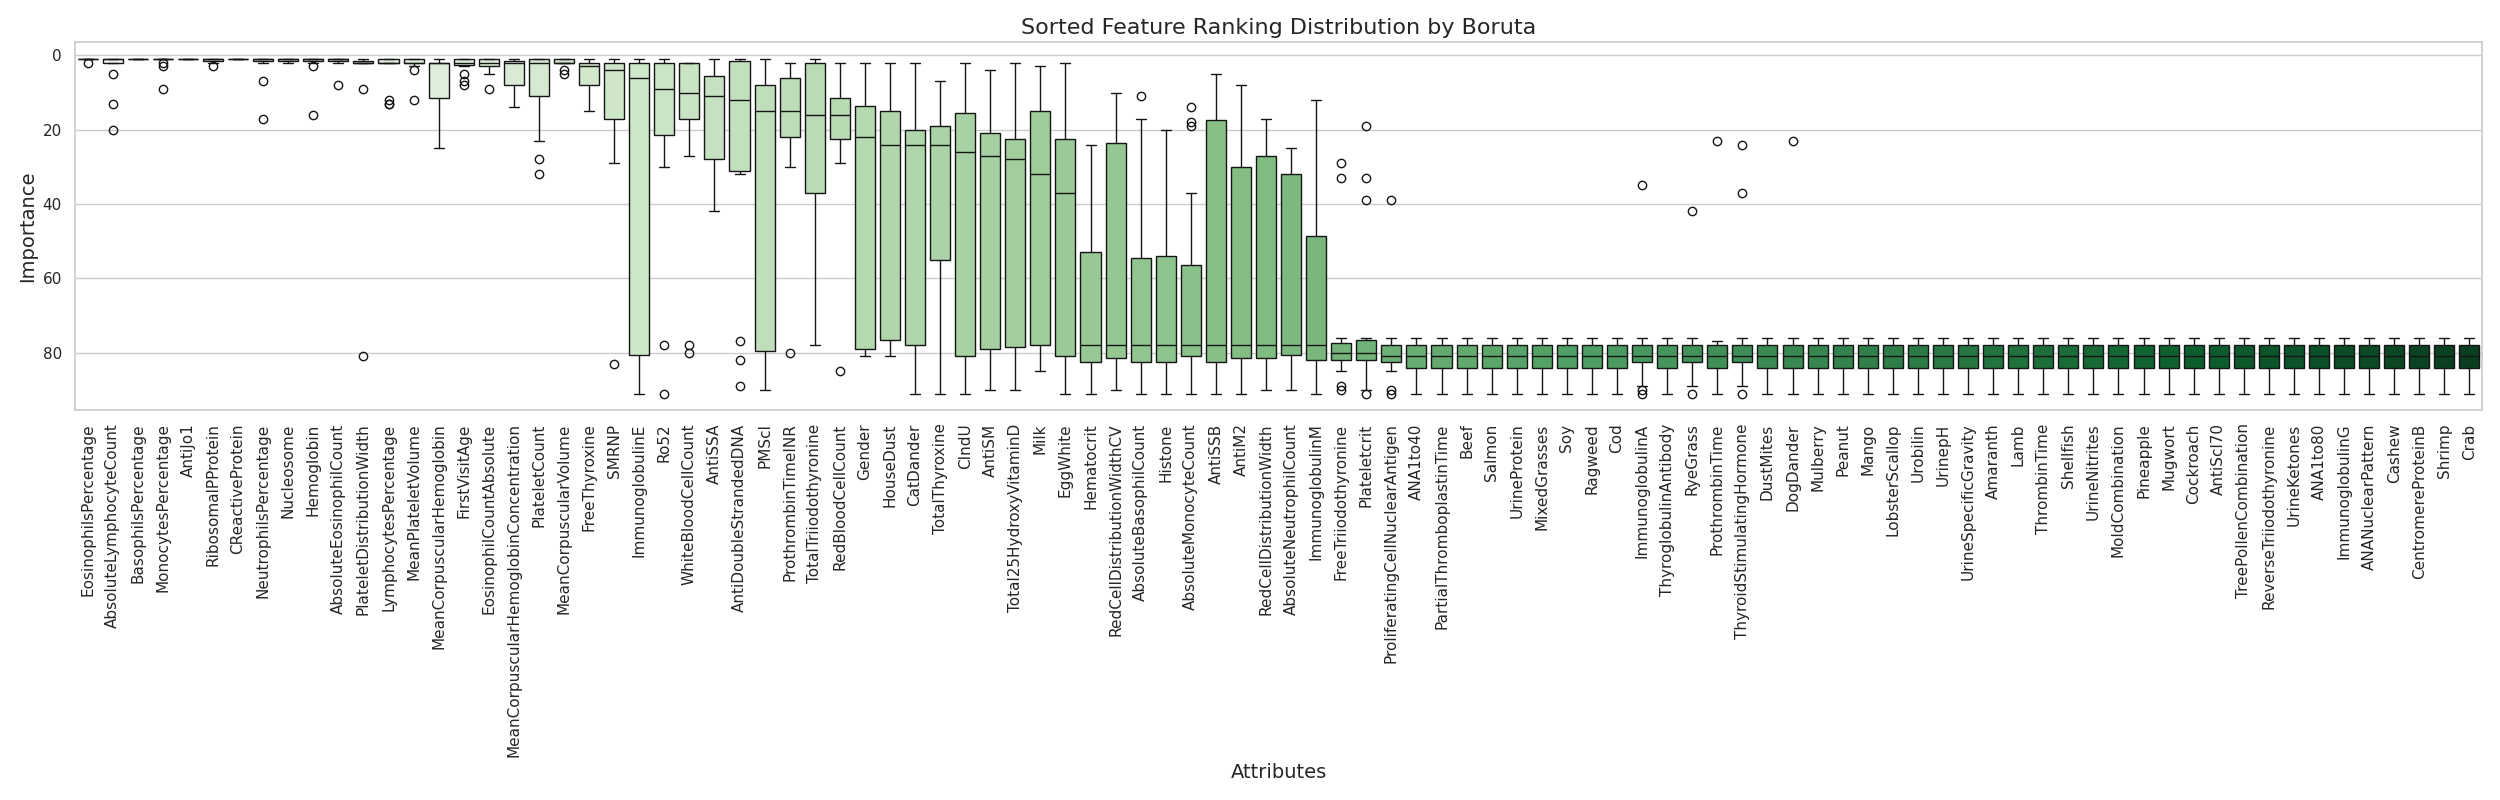
\includegraphics[width=\textwidth]{figures/boruta_by_group.png}
    %% Use \caption command for figure caption and label.
    \caption{Figure Caption}\label{Figure2}
    %% https://en.wikibooks.org/wiki/LaTeX/Importing_Graphics#Importing_external_graphics
\end{figure}


% insert image
\begin{figure}[t]%% placement specifier
    %% Use \includegraphics command to insert graphic files. Place graphics files in 
    %% working directory.
    \centering%% For centre alignment of image.
    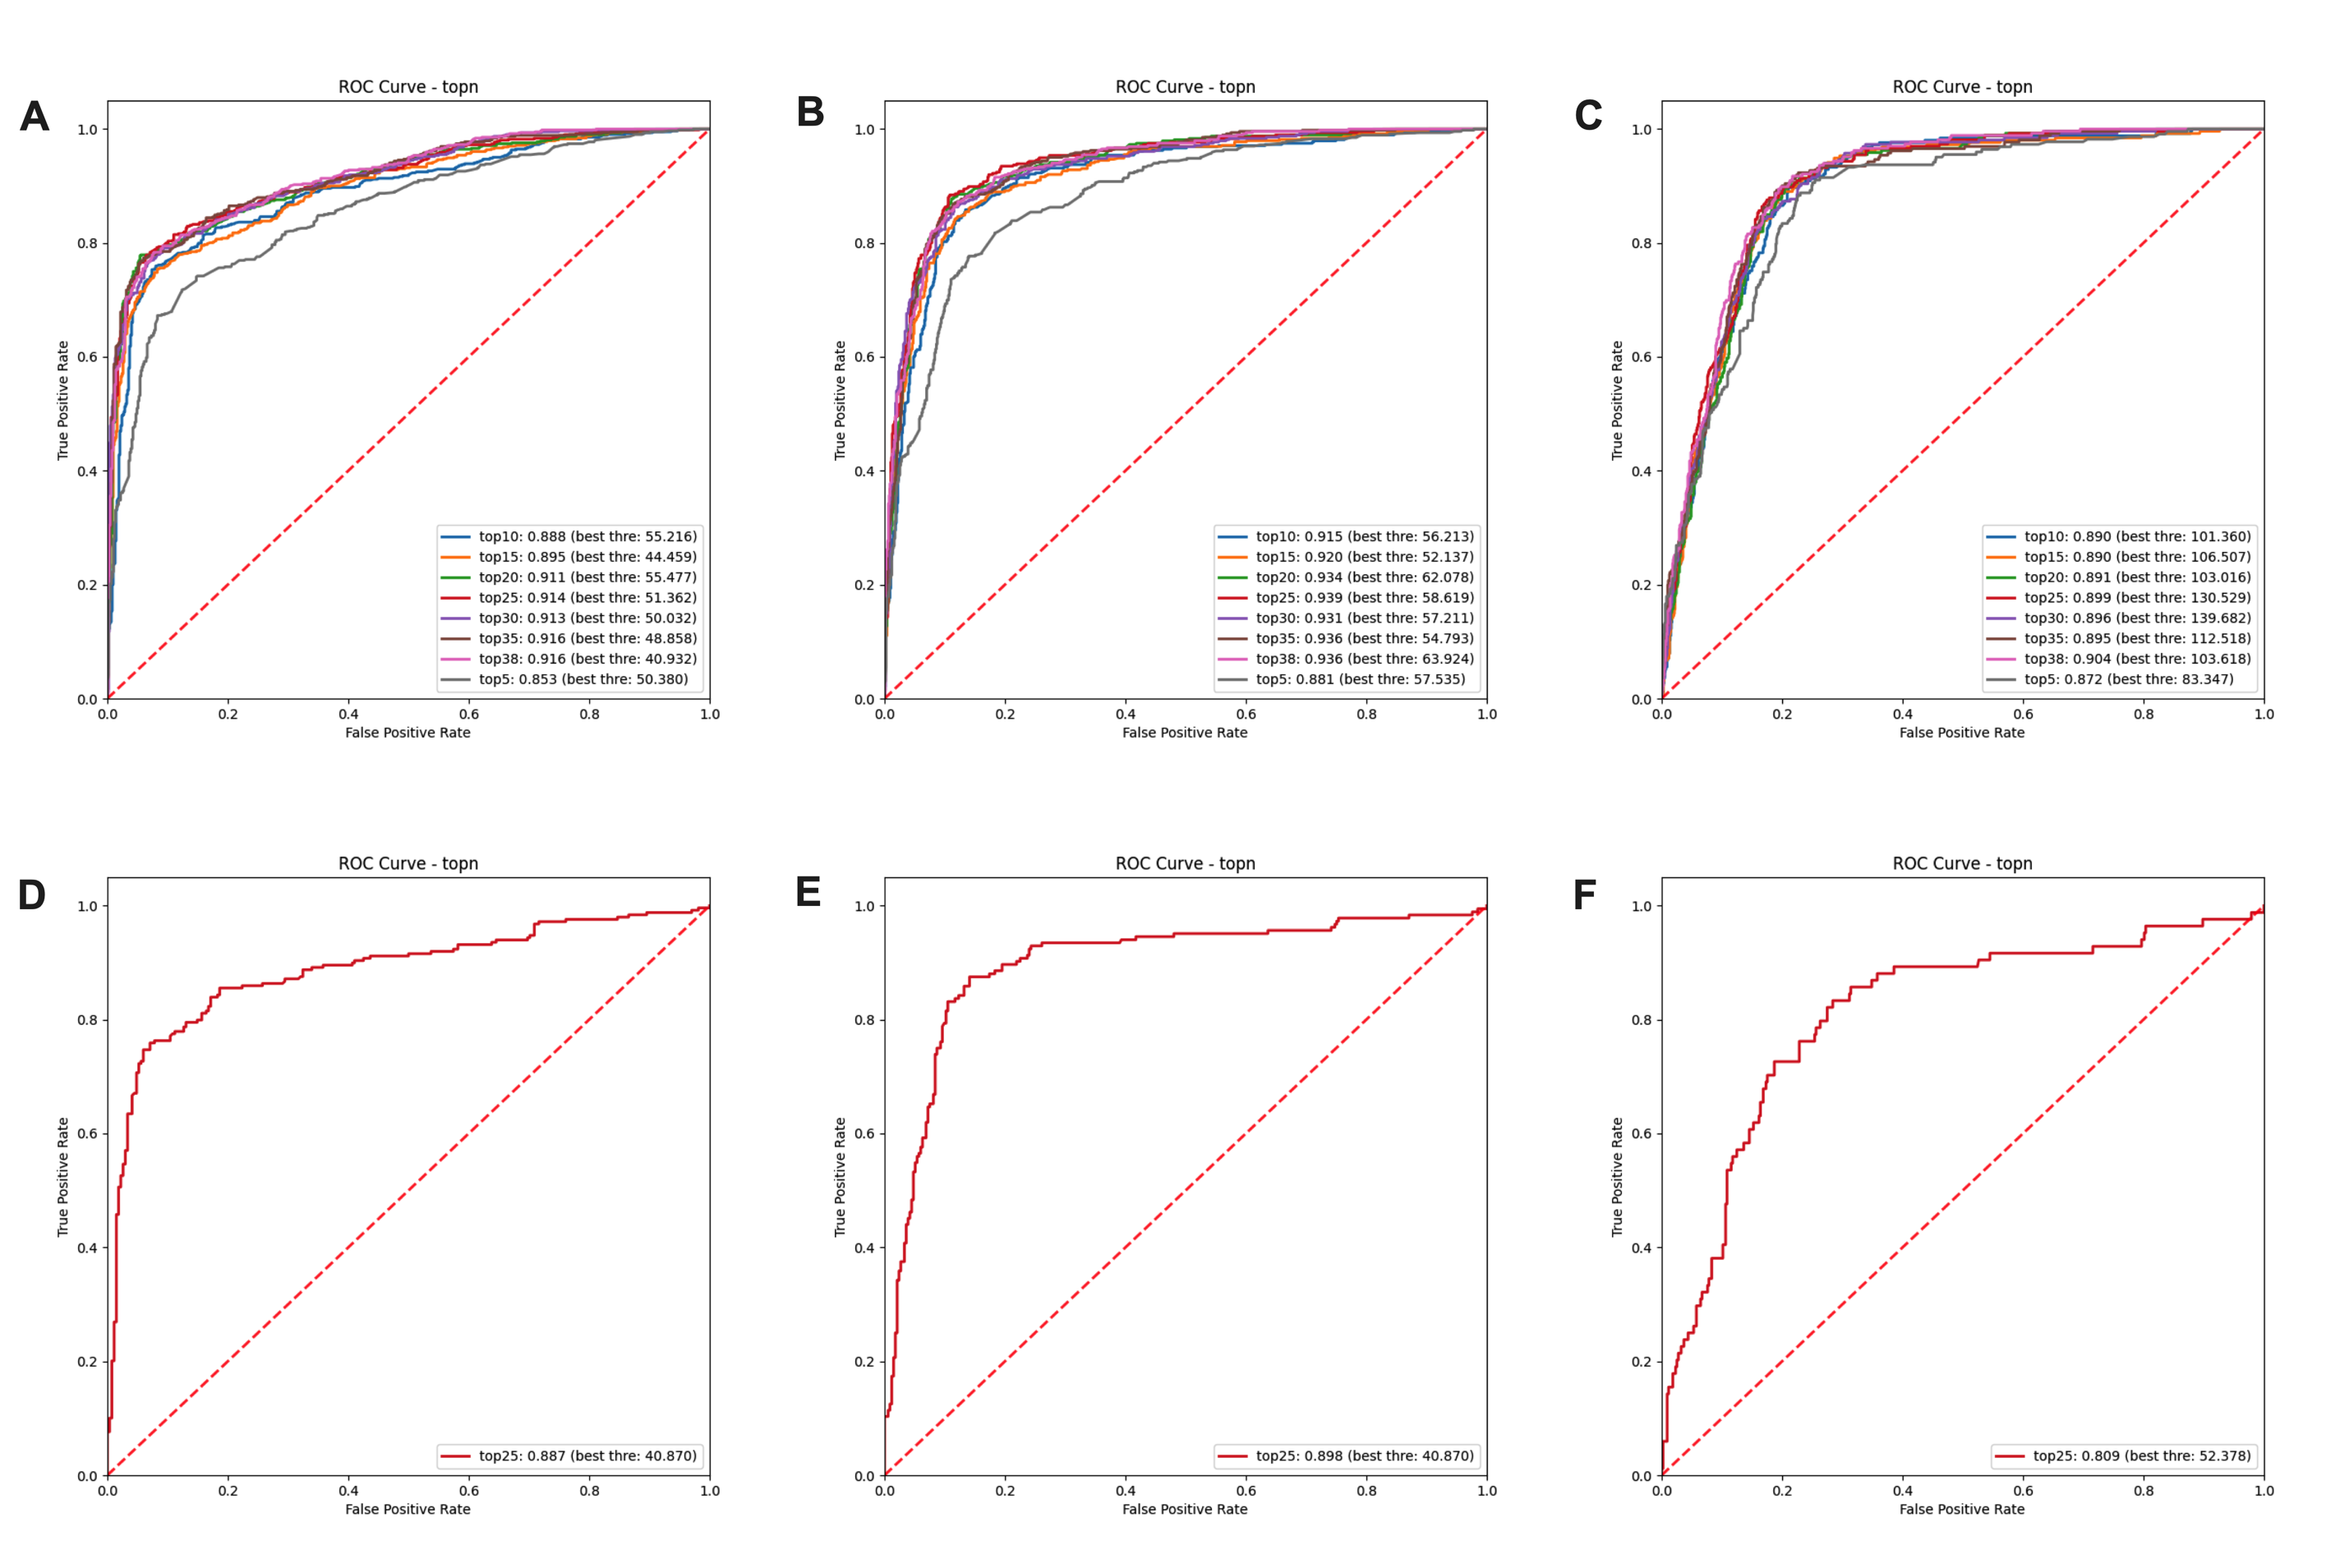
\includegraphics[width=\textwidth]{figures/topn_extval25.png}
    %% Use \caption command for figure caption and label.
    \caption{Figure Caption}\label{Figure3}
    %% https://en.wikibooks.org/wiki/LaTeX/Importing_Graphics#Importing_external_graphics
\end{figure}


\subsection{Model explanation}\label{ModelExplanationResults}





\section{Discussion}\label{Discussion}



Although the pathogenesis of CSU is not yet fully understood, it is well established that its signs and symptoms are due to the activation of mast cells and basophils, leading to the release of histamine and other inflammatory mediators\citep{Zuberbier2021The}. 

Based on recent evidence, it is known that the causes of CSU include autoimmunity Type I (CSUaiTI, or “autoallergic CSU”; with IgE autoantibodies to self-antigens) and autoimmunity Type IIb (CSUaiTIIb; with mast cell–directed activating autoantibodies). In CSU due to unknown cause (CSUuc), as of yet unknown mechanisms are relevant for the degranulation of skin mast cell (MC)\citep{sella2023type, Maronese2023IgG}.

The results of the basic tests performed in CSU can point to CSUaiTI vs CSUaiTIIb, with CRP more often elevated and eosinophil and basophil levels more often reduced in CSUaiTIIb\citep{Xiang2023Chronic}.
Other underlying causes include active thyroid disease, infections, inflammatory processes, food, and drugs but these can be both cause as well as only aggravating factor\citep{Kolkhir2021Autoimmune}


Eosinopenia in chronic spontaneous urticaria patients is associated with type IIb autoimmunity, high disease activity, and poor treatment response. \citep{Kolkhir2019Eosinopenia}, especially in children \citep{A2023Serum}.

Acute urticaria patients have abnormal cell immune responses, with lower numbers of CD3+ and CD4+ lymphocytes compared to healthy controls.\citep{De-yu2009Determination}.

Chronic idiopathic urticaria is associated with a prominent infiltrate of T-lymphocytes, monocytes, and mast cells, suggesting potential interactions between these cells to cause mediator release.\citep{Elias1986Studies}

Reducing thyroxine dose may cause flare-ups of chronic urticaria and angio-oedema, suggesting a possible link between thyroid function and musculoskeletal conditions.\citep{Dunkley2003Thyroid}

Mean platelet volume levels are higher in patients with chronic urticaria and correlate with its severity, suggesting coagulation and inflammation may play a role in the disease.\citep{Aleem2015Correlation} Chronic urticaria with a positive autologous serum skin test is associated with higher clinical severity, increased platelet volume, and increased C-reactive protein levels.\citep{Magen2010Increased} 

Neutrophilic urticarial dermatosis is a distinct cutaneous manifestation of neutrophilic aseptic disease, strongly associated with systemic diseases like Schnitzler syndrome, adult-onset Still disease, lupus erythematosus, and hereditary autoinflammatory fever syndromes.\citep{Kieffer2009Neutrophilic} Neutrophilic urticaria is common and not associated with other diseases, but its presence in biopsy samples may indicate rheumatic disease.\citep{Llamas‐Velasco2012Neutrophilic}





%% The Appendices part is started with the command \appendix;
%% appendix sections are then done as normal sections
\appendix
\section{Supplementary data}\label{sec:supplementary}

\href{run:supplementary/latex_data_description_table_train_test_origi.tex}{Supplementary Table1: Comparison of the characteristic between the training set and external testing set data in the time independent dataset}
\label{tab:train_test_origi}

\href{run:supplementary/latex_data_description_table_train_test_time.tex}{Supplementary Table2: Comparison of the characteristic between the training set and external testing set data in the time dependent dataset}
\label{tab:train_test_time}

\href{run:supplementary/kfolint_results.csv}{Supplementary Table 3: The discriminative performances of all 10 models in 5 fold cross validation}
\label{tab:kfold_results}

\href{run:supplementary/koldall.png}{Supplementary Figure 1: ROC curves of all 10 models in 5 fold cross validation}
\label{fig:kfold_all}

\href{run:supplementary/ranking_df.csv}{Supplementary Table 4: Feature importance ranking by Boruta algorithm}
\label{tab:boruta_ranking_df}

\href{run:supplementary/top38_confirmed_vars.csv}{Supplementary Table 5: 38 laboratory items confirmed as important by Boruta algorithm}
\label{tab:boruta_confirmed_vars}

\href{run:supplementary/extval_result.csv}{Supplementary Table 6: The performance of the final model on external test set}
\label{tab:extval_result}


\section{Acknowledgements}\label{Acknowledgements}


\bibliographystyle{elsarticle-harv} 
\bibliography{references}

 

\end{document}

\endinput



